\documentclass[10pt,twocolumn]{article} 
\usepackage{simpleConference}
\usepackage{times}
\usepackage{graphicx}
\usepackage{amssymb}
\usepackage{url,hyperref}
\usepackage{mathtools}

\begin{document}

\title{Advanced Real-time Reconstruction Methods}

\author{Conner Brooks\\
\\
CAP 4453\\
\today \\
\\
University of Central Florida\\
Orlando, FL, USA\\
\\
connerbrooks@gmail.com\\
}

\maketitle
\thispagestyle{empty}

\begin{abstract}
  The paper by Whelan et al. presents a new SLAM--
  Simultaneous Localization and Mapping--system capable of producing high quality
  reconstructions of an 3 dimensional environment with a low cost RGB-D sensor
  e.g. the Microsoft Kinect \ref{1}. This system is made possible by three
  key techniques.
  First, General-Purpose computing on Graphics Processing Units (GPGPU) and a 3D 
  cyclical buffer trick to extend the scanning volume to and unbounded spatial
  region. Second, this system also overcomes pose estimation limitations by combining
  dense geometric and photometric camera pose constraints. Third, the map of the 
  environment is updated according to place recognition and loop closure constraints.
  In this paper the first two techniques will be covered.
\end{abstract}

\section{Introduction}
3D reconstruction of environments is an important problem for 
robotics, virtual reality, and augmented reality. Understanding the geometry
allows a robot to avoid obticals and navigate, and with augmented reality
allows for interesting interactions with the environment. The advent of
commodity depth sensors has resulted in a large amount of reasearch 
concerning 3D understanding of environments. The work by Whelan et al. is the 
culmination of much of that work and represents one of the most advanced 
3D scanning systems. To understand the work presented in this paper, one must
first understand the work in the seminal paper by Newcombe et al. 

% TODO finish general intro

\subsection{Understanding Depth Sensors}

\section{Kinect Fusion Overview}

\subsection{Surface Measurement}

\begin{itemize}
\item At time $k$ raw depth map $R_k$--from kinect sensor--provides calibrated depth measurement $R_k(\mathbf{u}) \in \mathbb{R}$ at each image pixel $\mathbf{u} = (u,v)^{\top}$
\item Bilateral filter is applied $D_k(\mathbf{u})$. %\cite{kinect-fusion}
\item Filtered depth values are back projected into sensor frame of reference to obtain vertex map $\mathbf{V}_k$ where $\mathbf{V}_k(\mathbf{u}) = D_k(\mathbf{u})\mathbf{K}^{-1}\dot{\mathbf{u}}$, where $\mathbf{K}$ is the constant calibration matrix and transforms points $\rightarrow$ image pixels, and the dot denotes homogeneous vectors $mathbf{\dot{u}} := (\mathbf{u}^{\top}|1)^{\top}$
\item Since each frame is a measurment on a grid we can compute normal vectors with a cross product between neighboring map vertecies,\\ 
\end{itemize}
$\mathbf{N}_k(\mathrm{u}) = v[(\mathbf{V}_k(u+1,v) - \mathbf{V}_k(u, v)) \times (\mathbf{V}_k(u,v+1) - \mathbf{V}_k(u,v))]$, where $v[\mathbf{x}] = \mathbf{x} / \| \mathbf{x} \|_{2}$

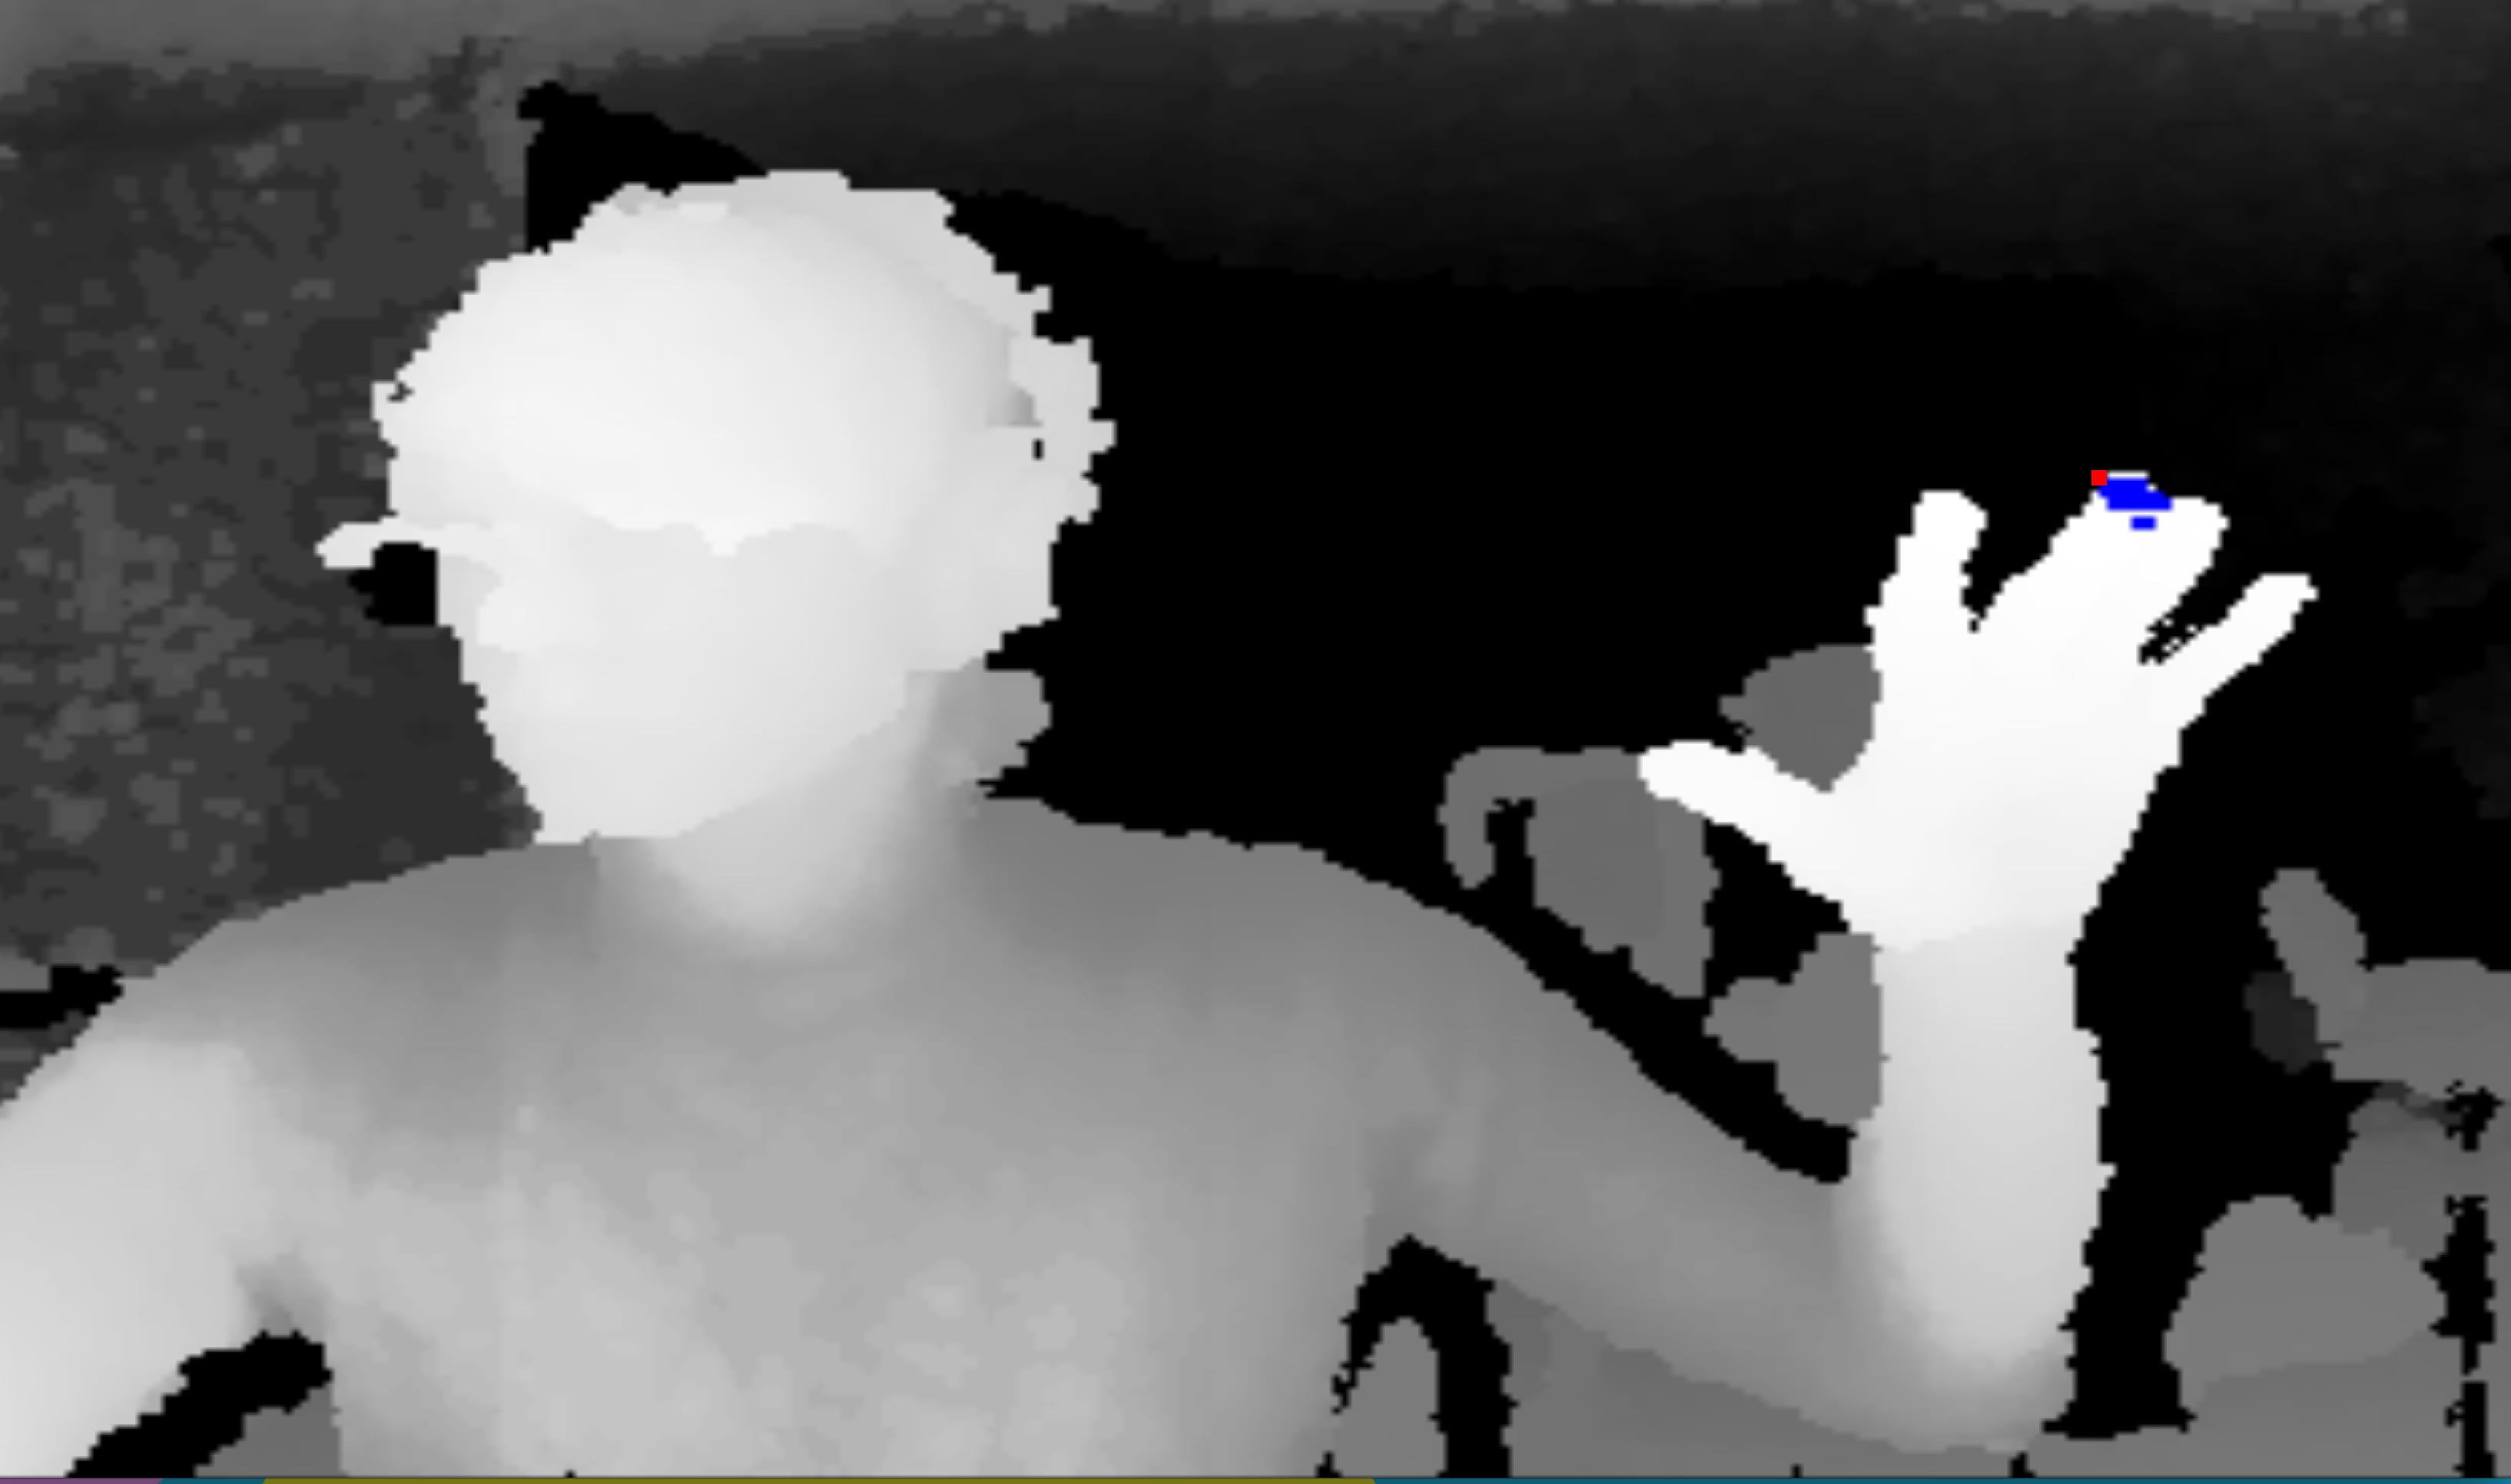
\includegraphics[width=0.8\linewidth]{depthimage}

\begin{itemize}
\item An $L = 3$ vertex and normal map pyrimid is computed.
\item Depth pyrimid $D^{l \in[1\dots L]}$ bottom is original bilateral filtered depth map. 
\item At each level $\textbf{V}^{l \in[1\dots L]}$ $\textbf{N}^{l \in[1\dots L]}$ with the equations from the previous slide.
\item Given the camera $\rightarrow$ global co-ordinate frame transform $\mathsf{T}_{g,k}$, the global frame vertex is $\textbf{V}^{g}_{k} = \mathsf{T}_{g,k} \dot{\textbf{V}}_{k}(\mathrm{u})$
\item The equivalent mapping of normal vectors $\mathbf{N}^{g}_{k}(\mathbf{u}) = \mathsf{R}_{g,k}\mathbf{N}(\mathbf{u})$
\end{itemize}

\subsection{Mapping as Surface Reconstruction}
  A signed distance functions value corresponds to the closest zero crossing (surface interface), taking positive values from surface $\rightarrow$ free space, and negative values on the non-visible side.
  The TSDF is denoted by $\mathbf{S}_{k}(\mathbf{p})$ where $\mathbf{p} \in \mathbb{R}^{3}$ is a global frame point in the TSDF with a specified resolution. The continous TSDF will be denoted by $\mathbf{S}$

\begin{figure}
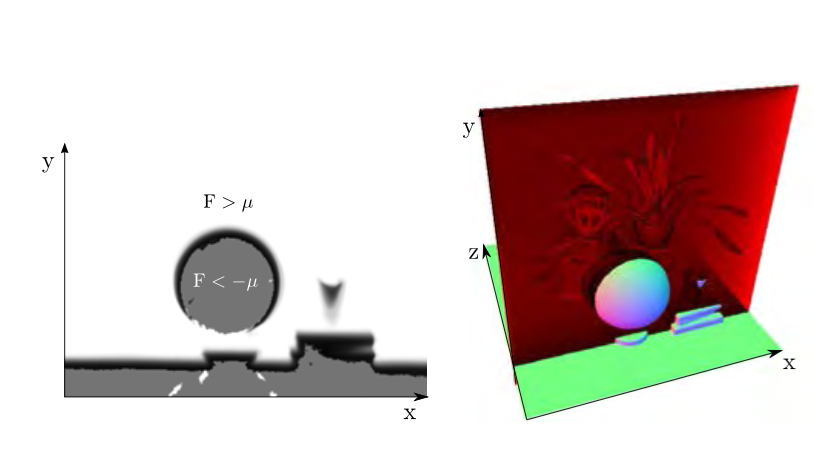
\includegraphics[width=0.8\linewidth]{tsdf}
\end{figure}

Two Components are stored at each location of the TSDF: the current truncated signed distance value $\mathrm{F}_{k}(\mathbf{p})$ and a weight $\mathrm{W}_k(\mathbf{p})$

$$
\mathbf{S}_{k} \rightarrow [\mathrm{F}_{k}(\mathbf{p}), \mathrm{W}_{k}(\mathbf{p})]
$$


\subsection{Surface Prediction from Ray Casting the TSDF}
We can compute a dense surface prediction by rendering the surface in a virtual camera with the current estimate $\mathsf{T}_{g,k}$. 

The surface prediction is stored as a vertex and normal map $\hat{\mathbf{V}}_{k}$ and $\hat{\mathbf{N}}_{k}$ and frame of reference $k$.

This is used in the subsequent camera pose estimation step.

In the global SDF, a per pixel raycast can be performed. Each ray $\mathsf{T}_{g,k}\mathbf{K}^{-1}\mathbf{\dot{u}}$ is marched starting from min depth for pixel and stopping at a zero crossing.

For points on or close to surface interface $F_{k}(\mathbf{p}) = 0$ we assume the gradient of the TSDF at $\mathbf{p}$ is orthogonal to the zero level set, so the surface normal for the associated pixel $\mathbf{u}$ can be computed directly from $F_{k}$ using a numerical derivative of the SDF:
$$
\mathsf{R}_{g,k} \mathbf{\hat{N}}_{k} (\mathbf{u}) = \mathbf{\hat{N}}^{g}_{k} = v[\nabla F(\mathbf{p})], \nabla F = 
\begin{bmatrix}
    \frac{\delta F}{\delta x}, & \frac{\delta F}{\delta y}, & \frac{\delta F}{\delta z}
\end{bmatrix}^{\top}
$$


\subsection{Sensor Pose Estimation}
The live 6DOF camer pose estimated for a frame at time k
$$
\mathsf{T}_{g,k} = 
\begin{bmatrix}
  \mathsf{R}_{g,k} & \mathbf{t}_{g,k} \\
  0 & 1
\end{bmatrix}
\in \mathbb{SE}_{3}
$$

where $\mathbb{SE}_{3} := \{\mathsf{R}, \mathbf{t}\ |\ \mathsf{R} \in \mathbb{SO}_{3}, \mathbf{t} \in \mathbb{R}^{3}\}$

\hfill \break

To track the sensor frame, the live surface measurement $(\mathbf{V}_{k}, \mathbf{N}_{k})$ against the model prediction from the previous frame $(\mathbf{\hat{V}}_{k-1}, \mathbf{\hat{N}}_{k-1})$

First we must find correspondences between the two sets of points with projective data association. 
\begin{figure}
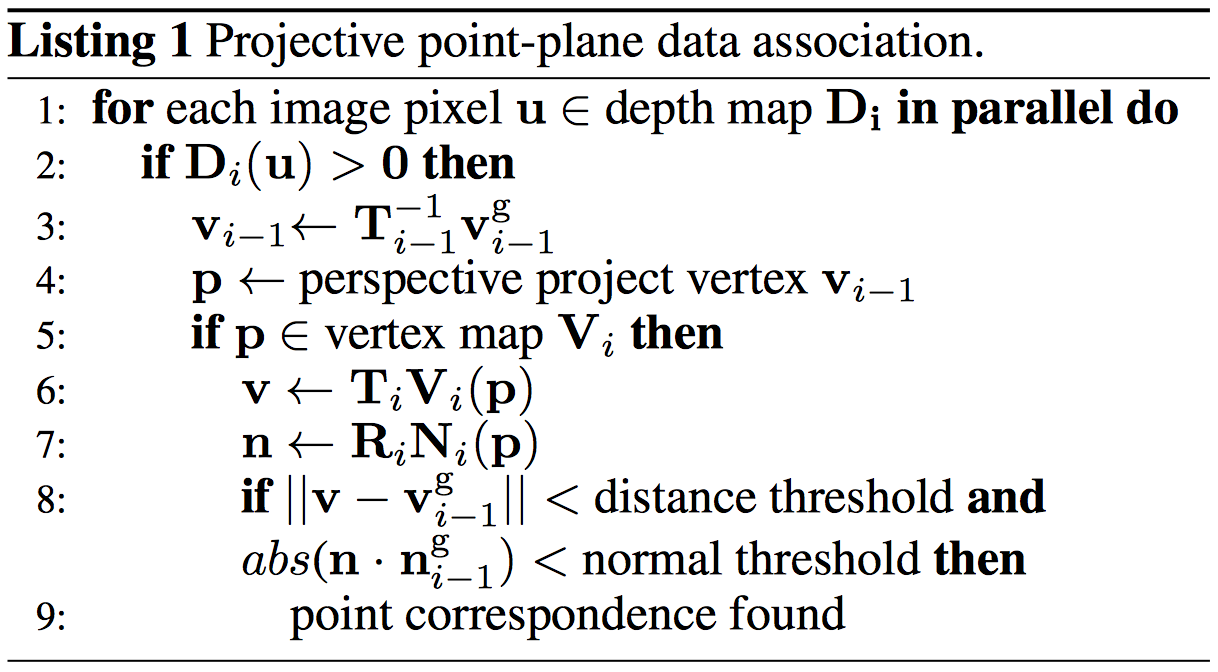
\includegraphics[width=0.8\linewidth]{icp}
\end{figure}


Given these correspondences the output of each ICP iteration is a single transformation matrix $T$ which minimizes the point to plane error metric, or the sum of squared distances between each point in the current frame and the tangent plane at corresponding points in the previous frame.

$$
\mathbf{E}(\mathsf{T}_{g,k}) = 
\sum_{\substack{
   \mathbf{u} \in \mathcal{U} \\
   \Omega_{k}(\mathbf{u}) \neq null
  }}
  \| ( \mathsf{T}_{g,k} \mathbf{\dot{V}} (\mathbf{u}) - \mathbf{\hat{V}}^{g}_{k-1} (\mathbf{\hat{u}}))^{\top} \mathbf{\hat{N}}^{g}_{k-1} (\mathbf{\hat{u}}) \|_{2}
$$

A linear approximation is used to solve this system, we assume that the transformation between two frames is incremental.

\begin{figure}
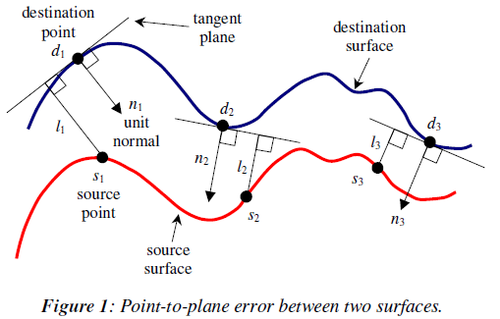
\includegraphics[width=0.8\linewidth]{pointplane}
\end{figure}

\begin{figure}
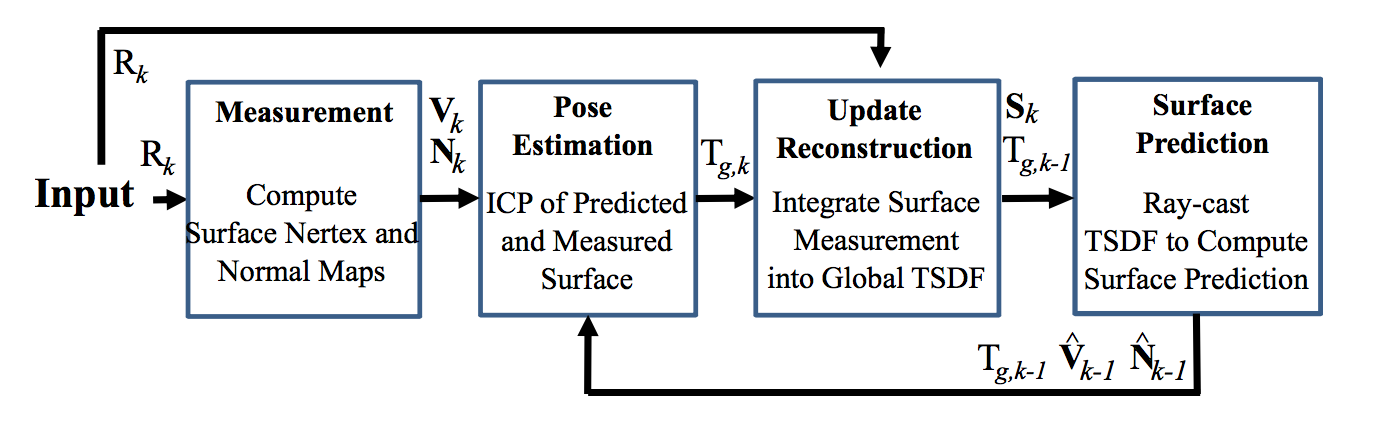
\includegraphics[width=0.8\linewidth]{workflow}
\end{figure}

\begin{figure}
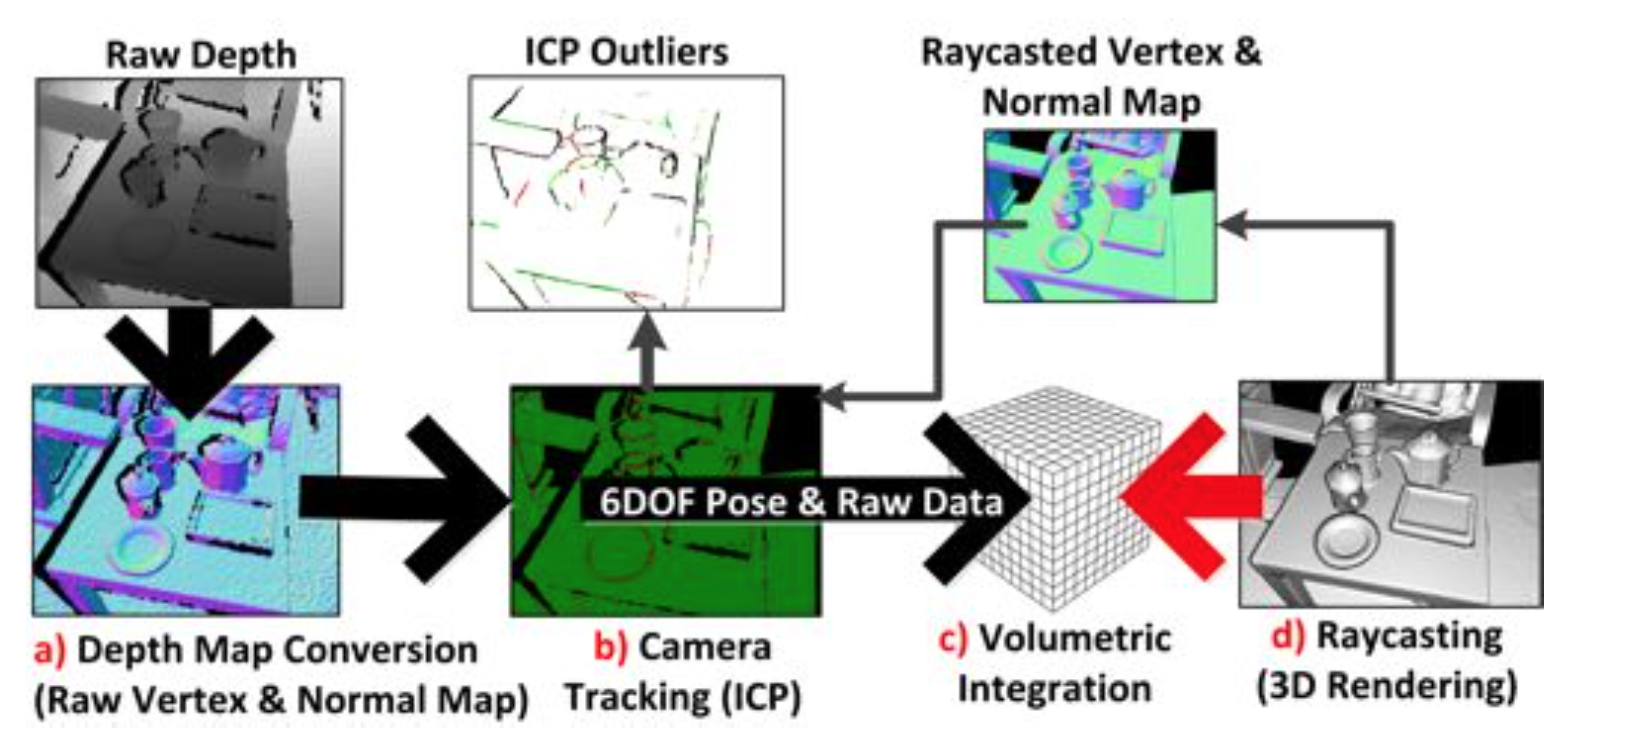
\includegraphics[width=0.8\linewidth]{kinectfusion}
\end{figure}




\section{Extensions to Kinect Fusion}

\subsection{Cyclical Buffer Trick}
The position of the TSDF volume in the global frame is initially $\mathbf{g}_{0} = (0, 0, 0)^{\top}$

When our pose estimate leaves a movement threshold $m_{s}$ around $\mathbf{g}_{i}$ will cause a volume shift.
The shift triggers and the TSDF is virtually translated about the camera pose (in voxel units) to bring the camera's position to $\mathbf{g}_{i+1}$.


To compute the new camera pose, we must compute the number of voxel units crossed

$$
u = \lfloor \frac{v_{s}t^{T}_{i+1}}{v_d} \rfloor
$$

then shift the pose, updating the global position of the TSDF,

$$
\mathbf{t}^{T'}_{i+1} = \mathbf{t}^{T}_{i+1} - \frac{v_{d}\mathbf{u}}{v_{s}}
$$

$$
\mathbf{g}_{i+1} = \mathbf{g}_{i} + \mathbf{u}
$$



\subsection{Photometric Camera Pose Estimation}
Given two consecutive RGB-D frames $[\mathbf{rgb}_{n-1}, \mathbf{d}_{n-1}]$ and $[\mathbf{rgb}_{n}, \mathbf{d}_{n}]$

A rigid transform is computed between the two that maximizes photo-consistency. 
We define $V: \Omega \rightarrow \mathbb{R}^{3}$ to be back-projection of point $\mathbf{p}$ dependent on
a metric depth map $M: \Omega \rightarrow \mathbb{R}$ and
a camera intrinsics matrix $\mathbf{K} \rightarrow$ principle points $c_{x}, c_{y}$ and focal lengths $f_{x}, f_{y}$ 

$$
V(\mathbf{p}) = \left( \frac{(\mathbf{p}_{x} - c_{x})M(\mathbf{p})}{f_{x}}, \frac{(\mathbf{p}_{y} - c_{y})M(\mathbf{p})}{f_{y}}, M(\mathbf{p}) \right)^{\top}
$$

A perspective projection of a 3D point $\mathbf{v} = (x,y,z)^{\top}$ is defined, as well as a dehomogenization by $\Pi(\mathbf{v}) = (x/z, y/z)^{\top}$. The cost to be minimised depends on the difference in intensity values between the two images $I_{n-1}, I{n}: \Omega \rightarrow \mathbb{N}$

$$
\mathbf{E}_{rgbd} = 
\sum_{\substack{
   \mathbf{p} \in \mathcal{L} 
  }}
  \| I_{n}(\mathbf{p} - I_{n-1}(\Pi_{n-1}(exp(\xi)\mathbf{T}V_{n}(\mathbf{p})))  \|^{2}
$$

where $\mathcal{L}$ is the list of valid interest points populated by the following alogrithm and $\mathbf{T}$ is the current estimate of the transform.

\subsection{Combined Camera Pose Estimation}

$$
E = E_{icp} + w_{rgbd}E_{rgbd}
$$

where $w_{rgbd}$ is the weight and was set empirically to 0.1 to refelect the difference in metrics used for ICP and RGBD costs.

For each step a linear least-squares problem  is minimized by solving:
% TODO least squares equation
$$
$$




\bibliographystyle{abbrv}
\bibliography{refs}
\end{document}
